\documentclass[a4paper, 12p]{article}
\usepackage[pdftex, hidelinks]{hyperref}

\usepackage{bm}
\usepackage{xcolor}
\usepackage[T1]{fontenc}
\usepackage[utf8]{inputenc}
\usepackage{algorithmic}
\usepackage{algorithm}
\usepackage{amsfonts}
\usepackage{amssymb}
\usepackage{courier}
\usepackage{booktabs}
\usepackage{graphicx}
\usepackage{listings}
\usepackage{mathtools}
\usepackage{amssymb}
\lstset{basicstyle=\footnotesize\ttfamily,
breakatwhitespace = false,
breaklines = true,
keepspaces = true,
language = R,
showspaces = false,
showstringspaces = false,
belowcaptionskip = \bigskipamount,
framerule = 0.80pt,
frame = tb,
belowskip = \bigskipamount,
escapeinside={<@}{@>}}

\title{TDDE01 -- Machine Learning \\
Laboration Report 6}
\author{{Martin Estgren \texttt{<mares480>}} \\
{Linköping University (LiU), Sweden}}

\begin{document}
\pagenumbering{arabic}
    \maketitle % Generate.
    
    For this assignment we will examine how a \textit{neural net} can be used to approximate the \textit{sinusoidal function} with \textit{resilient back propagation} using the \textit{batched gradient descent function} (equation:\ref{eq:batch_gradient}). The \textit{neural net} will consist of one hidden layer with 10 \textit{perceptions} (equation:\ref{eq:perceptron}), all using the \textit{logistic function} (equation:\ref{eq:logistic}) as \textit{activation function}. 

   \begin{equation} \label{eq:logistic}
        f(x) = \frac{1}{1 + e^{-k(x-x_0)}}
    \end{equation}

    \begin{equation} \label{eq:batch_gradient}
        \bm{w}_{(i)} = \bm{w}_{(i-1)} - \eta_k \nabla E(\bm{w}_{(i-1)})
    \end{equation}

    \begin{equation} \label{eq:perceptron}
        \hat{y}_j(\bm{x}) = \sigma(w_0 + \sum_{h=1}^{H} \sigma(w_{0h} + \bm{w}_h^\intercal\bm{x}))
    \end{equation}

    First a sample data set is generated from a uniform random distribution in the range \(0...10\), 50 samples are generated and the sinusoidal value stored as for evaluation and training. THe set of 50 observations are then split into one training set and one validation set of equal size.

    \lstinputlisting[firstline=4, lastline=8]{share/assignment.r}

    To find the best \textit{neural net} we create 10 nets with different \textit{threshold} as and initial weights set as uniform random samples between -1 and 1. For each of the nets the \textit{means squared error} (M.S.E) is calculated with the validation data set. 

    \lstinputlisting[firstline=12, lastline=17]{share/assignment.r}

    The best net is selected and re-run on the entire generated data set. For this data set the optimal threshold was found to be 0.004. 

    \lstinputlisting[firstline=18, lastline=19]{share/assignment.r}

    The resulting prediction of the net can be seen in figure~\ref{fig:predictions} and a visual representation of the best neural net in figure~\ref{fig:network}.

    \begin{figure}[H]
        \centering
        \caption{(Poor) Visual representation of the best neural network.}
        \label{fig:network}
        
\includegraphics[width=0.75\textwidth]{share/network.eps}
    \end{figure}
    The figure above shows a graph representation of the neural net. The black numbers are the individual weights and the blue ones are the intercept for each node.

    \begin{figure}[H]
        \centering
        \caption{Neural net predictions, the red values are the predictions and the black predicted.}
        \label{fig:predictions}
        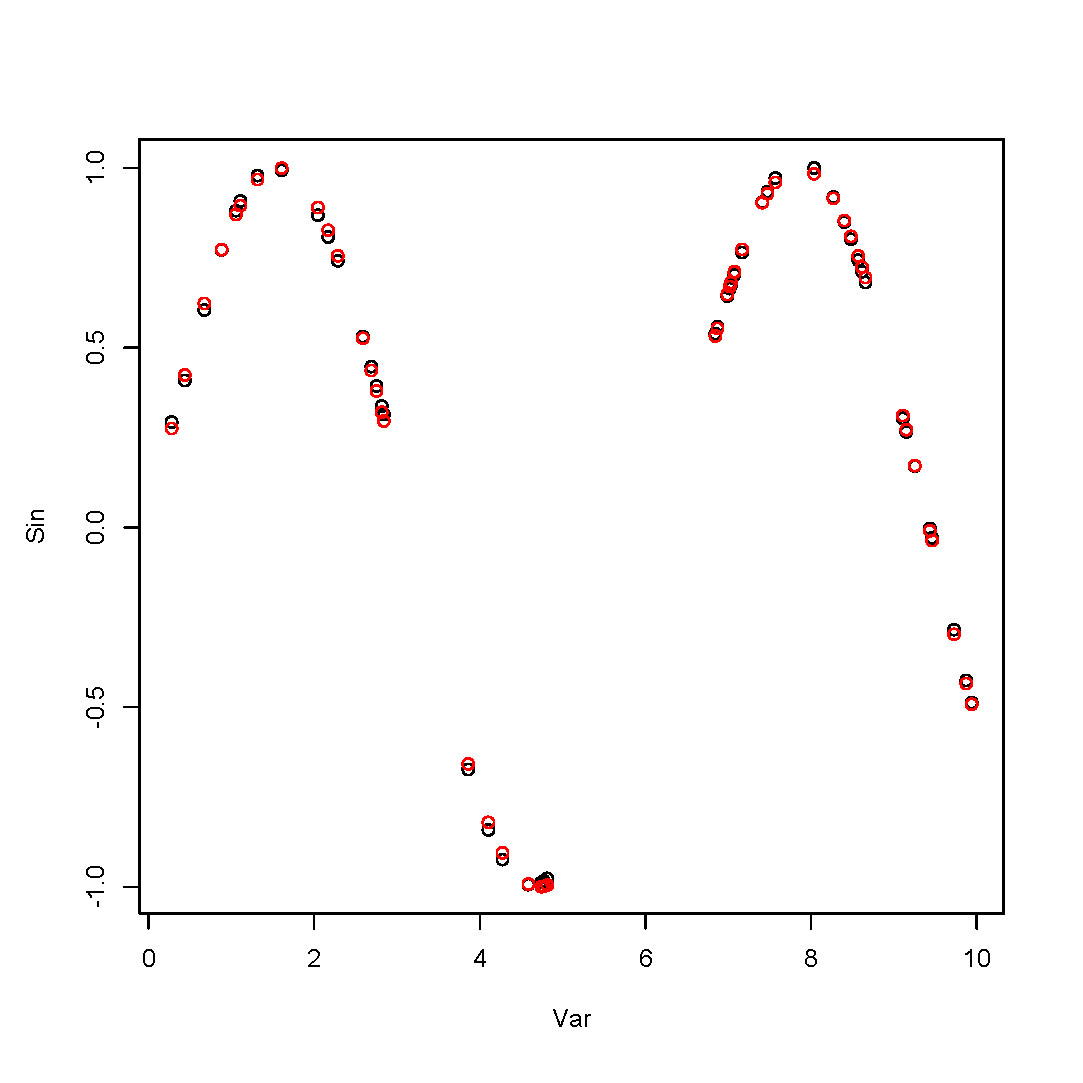
\includegraphics[width=\textwidth]{share/predictions.eps}
    \end{figure}
    The resulting predictions are very close the ones in the original data, indicating that the neural net has produced a good approximation of the sinusoidal function.

    The full code for this assignment can be found in the appendix on the next page.

    \nocite{*} % No warnings.
    \bibliographystyle{alpha}
    \bibliography{report}
    \onecolumn \appendix
    \section*{Appendix}

    \lstinputlisting[caption={Code for the assignment}, label={lst:properties}]{share/assignment.r}

\end{document}
